\chapter{Appendix}
\label{ch:appendix}

\section{Hyperparameter Search Spaces}
\label{app:hyperparams}

\begin{table}[H]
\centering
\caption{Hyperparameter search spaces used in RandomizedSearchCV (20 iterations, 5-fold GroupKFold on training sessions only).}
\label{tab:hp_search}
\begin{tabular}{lll}
\toprule
\textbf{Model} & \textbf{Parameter} & \textbf{Search space} \\
\midrule
Logistic Regression & \texttt{clf\_\_C}                   & $\{0.01, 0.1, 1, 10, 100\}$ \\
\midrule
\multirow{3}{*}{Random Forest}
                    & \texttt{clf\_\_n\_estimators}       & $\{100, 200, 500\}$ \\
                    & \texttt{clf\_\_max\_depth}          & $\{5, 10, 20, \texttt{None}\}$ \\
                    & \texttt{clf\_\_min\_samples\_leaf}  & $\{1, 2, 5\}$ \\
\midrule
\multirow{4}{*}{XGBoost}
                    & \texttt{clf\_\_n\_estimators}       & $\{200, 500\}$ \\
                    & \texttt{clf\_\_learning\_rate}      & $\{0.05, 0.1, 0.2\}$ \\
                    & \texttt{clf\_\_max\_depth}          & $\{4, 6, 8\}$ \\
                    & \texttt{clf\_\_subsample}           & $\{0.8, 1.0\}$ \\
\midrule
\multirow{2}{*}{SVM}
                    & \texttt{clf\_\_C}                   & $\{0.01, 0.1, 1, 10\}$ \\
                    & \texttt{clf\_\_gamma}               & $\{\texttt{scale}, \texttt{auto}\}$ \\
\bottomrule
\end{tabular}
\end{table}

\section{Per-Fold Diagnostics on the Campus Dataset}
\label{app:fold_diagnostics}

\Cref{tab:fold_quality_campus} is referenced from \Cref{sec:res_campus} to explain the per-class $F_1$ collapse of \texttt{cobblestone} and \texttt{muddy\_dirt\_track} on the five-class campus problem.

\begin{table}[H]
\centering
\caption{Per-fold, per-class diagnostics on the campus dataset under LORO-CV. \textit{Train n} and \textit{Test n} are window counts in the training and held-out partitions for that fold; \textit{Count} is flagged \texttt{LOW} when the training-fold count for that class falls below the threshold used by the diagnostic (here, $\approx 50$ windows), signalling that the model has very little material to learn the class from. \textit{Speed TVD} is the total variation distance between the train- and test-fold per-class speed-bin distributions; \textit{Speed} is flagged \texttt{WARN} when the train and test speed distributions diverge substantially ($\mathrm{TVD} > 0.4$) and \texttt{N/A} when the test fold contains no windows of that class. Source: \texttt{results/Campus/fold\_quality\_diagnostics.csv}.}
\label{tab:fold_quality_campus}
\small
\renewcommand{\arraystretch}{1.05}
\begin{tabular}{llrrcrc}
\toprule
\textbf{Test fold} & \textbf{Class} & \textbf{Train $n$} & \textbf{Test $n$} & \textbf{Count} & \textbf{Speed TVD} & \textbf{Speed} \\
\midrule
\multirow{5}{*}{23 Feb}
  & cobblestone         & 355 & 0   & OK  & ---   & N/A  \\
  & dry\_dirt\_track    & 652 & 0   & OK  & ---   & N/A  \\
  & grass               & 462 & 26  & OK  & 0.058 & OK   \\
  & muddy\_dirt\_track  & 46  & 99  & LOW & 0.727 & WARN \\
  & smooth\_terrain     & 538 & 168 & OK  & 0.559 & WARN \\
\midrule
\multirow{5}{*}{26 Feb}
  & cobblestone         & 355 & 0   & OK  & ---   & N/A  \\
  & dry\_dirt\_track    & 652 & 0   & OK  & ---   & N/A  \\
  & grass               & 444 & 44  & OK  & 0.151 & OK   \\
  & muddy\_dirt\_track  & 99  & 46  & OK  & 0.727 & WARN \\
  & smooth\_terrain     & 651 & 55  & OK  & 0.622 & WARN \\
\midrule
\multirow{5}{*}{9 Mar (A)}
  & cobblestone         & 355 & 0   & OK  & ---   & N/A  \\
  & dry\_dirt\_track    & 258 & 394 & OK  & 0.208 & OK   \\
  & grass               & 420 & 68  & OK  & 0.139 & OK   \\
  & muddy\_dirt\_track  & 145 & 0   & OK  & ---   & N/A  \\
  & smooth\_terrain     & 504 & 202 & OK  & 0.464 & WARN \\
\midrule
\multirow{5}{*}{9 Mar (B)}
  & cobblestone         & 318 & 37  & OK  & 0.865 & WARN \\
  & dry\_dirt\_track    & 394 & 258 & OK  & 0.208 & OK   \\
  & grass               & 240 & 248 & OK  & 0.060 & OK   \\
  & muddy\_dirt\_track  & 145 & 0   & OK  & ---   & N/A  \\
  & smooth\_terrain     & 585 & 121 & OK  & 0.515 & WARN \\
\midrule
\multirow{5}{*}{26 Mar}
  & cobblestone         & 37  & 318 & LOW & 0.865 & WARN \\
  & dry\_dirt\_track    & 652 & 0   & OK  & ---   & N/A  \\
  & grass               & 386 & 102 & OK  & 0.099 & OK   \\
  & muddy\_dirt\_track  & 145 & 0   & OK  & ---   & N/A  \\
  & smooth\_terrain     & 546 & 160 & OK  & 0.200 & OK   \\
\bottomrule
\end{tabular}
\end{table}

\newpage
\section{Transition-Detection Diagnostic Figures}
\label{app:transition_figures}

This appendix collects three diagnostic traces referenced from \Cref{sec:res_transition}. \Cref{fig:transition_timelines} shows the per-window Random Forest posterior on a representative farm run with the implicit $n_{\text{stable}} = 5$ detections overlaid; \Cref{fig:cusum_timeline} shows the same posterior together with the running CUSUM statistics $g_c(k)$ and the threshold crossings; \Cref{fig:transition_timelines_c} shows the same implicit-detector view on a representative campus run.

\begin{figure}[H]
    \centering
    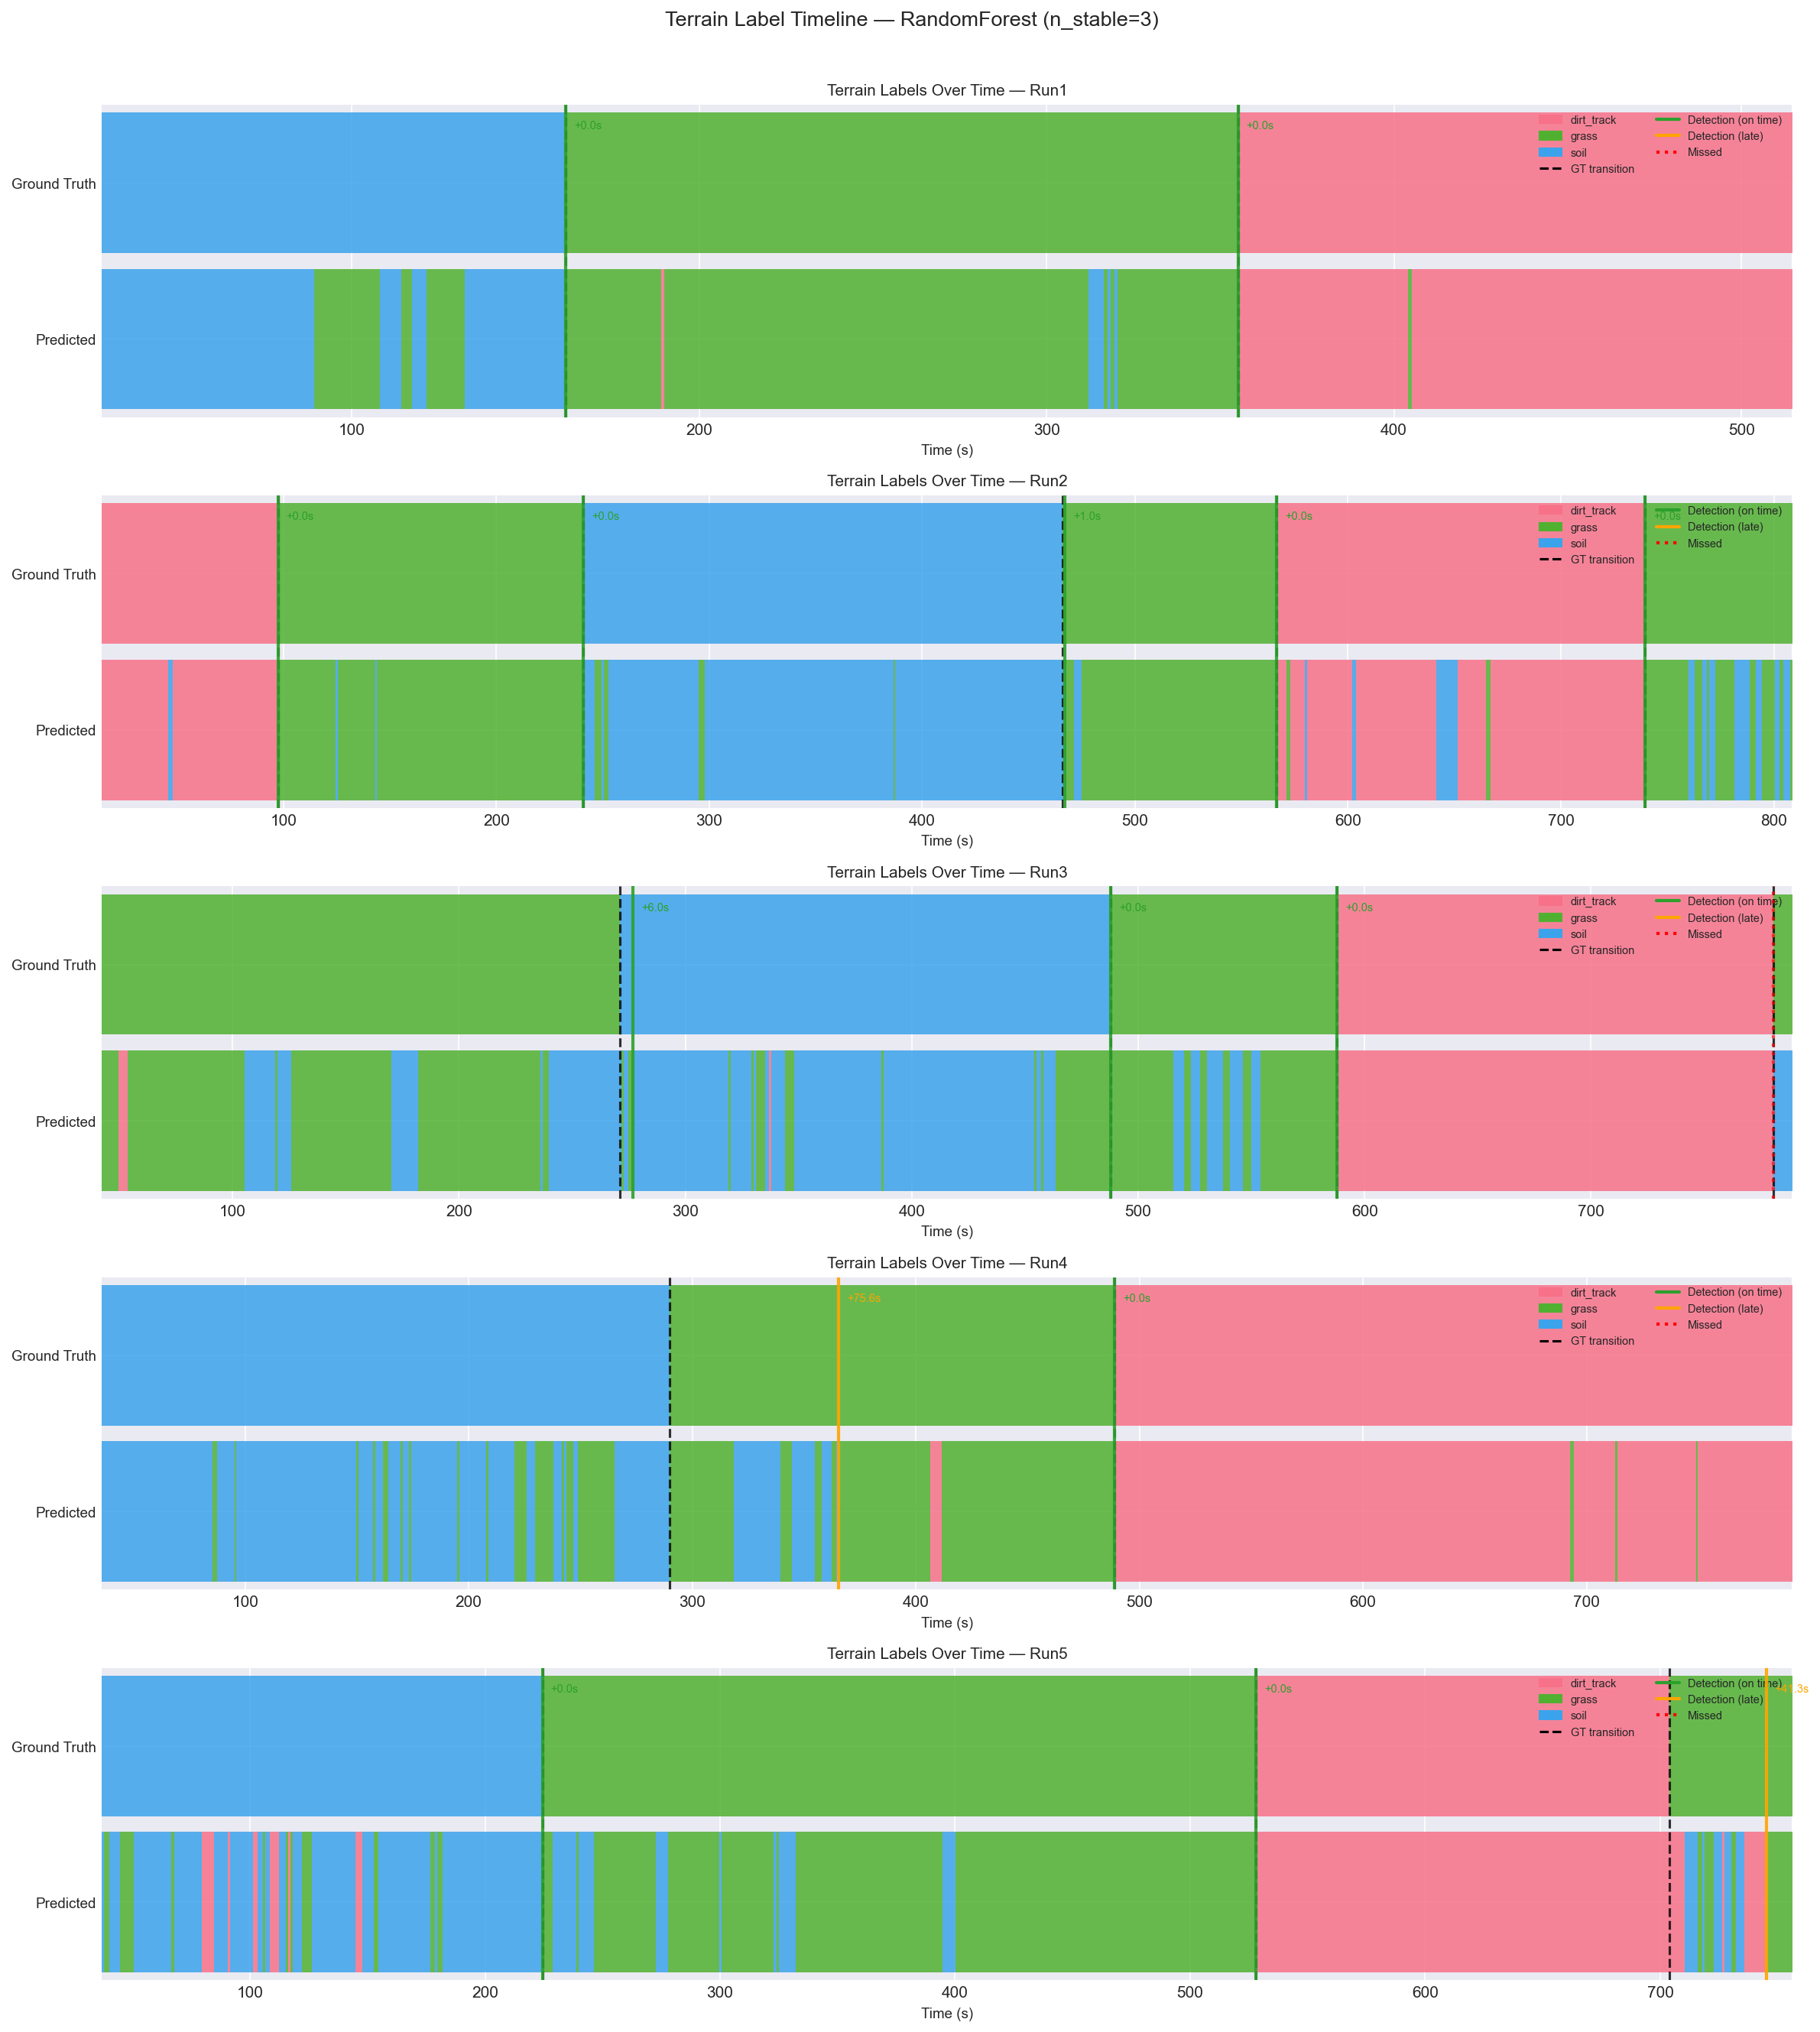
\includegraphics[width=0.85\textwidth]{Pictures/Figures/transition_timelines_randomforest_f.png}
    \caption{Random Forest per-window posterior on a representative farm run, with the $n_{\text{stable}} = 5$ detections overlaid. Shaded bands are ground-truth class segments; vertical lines mark the implicit detector's alarms.}
    \label{fig:transition_timelines}
\end{figure}

\begin{figure}[H]
    \centering
    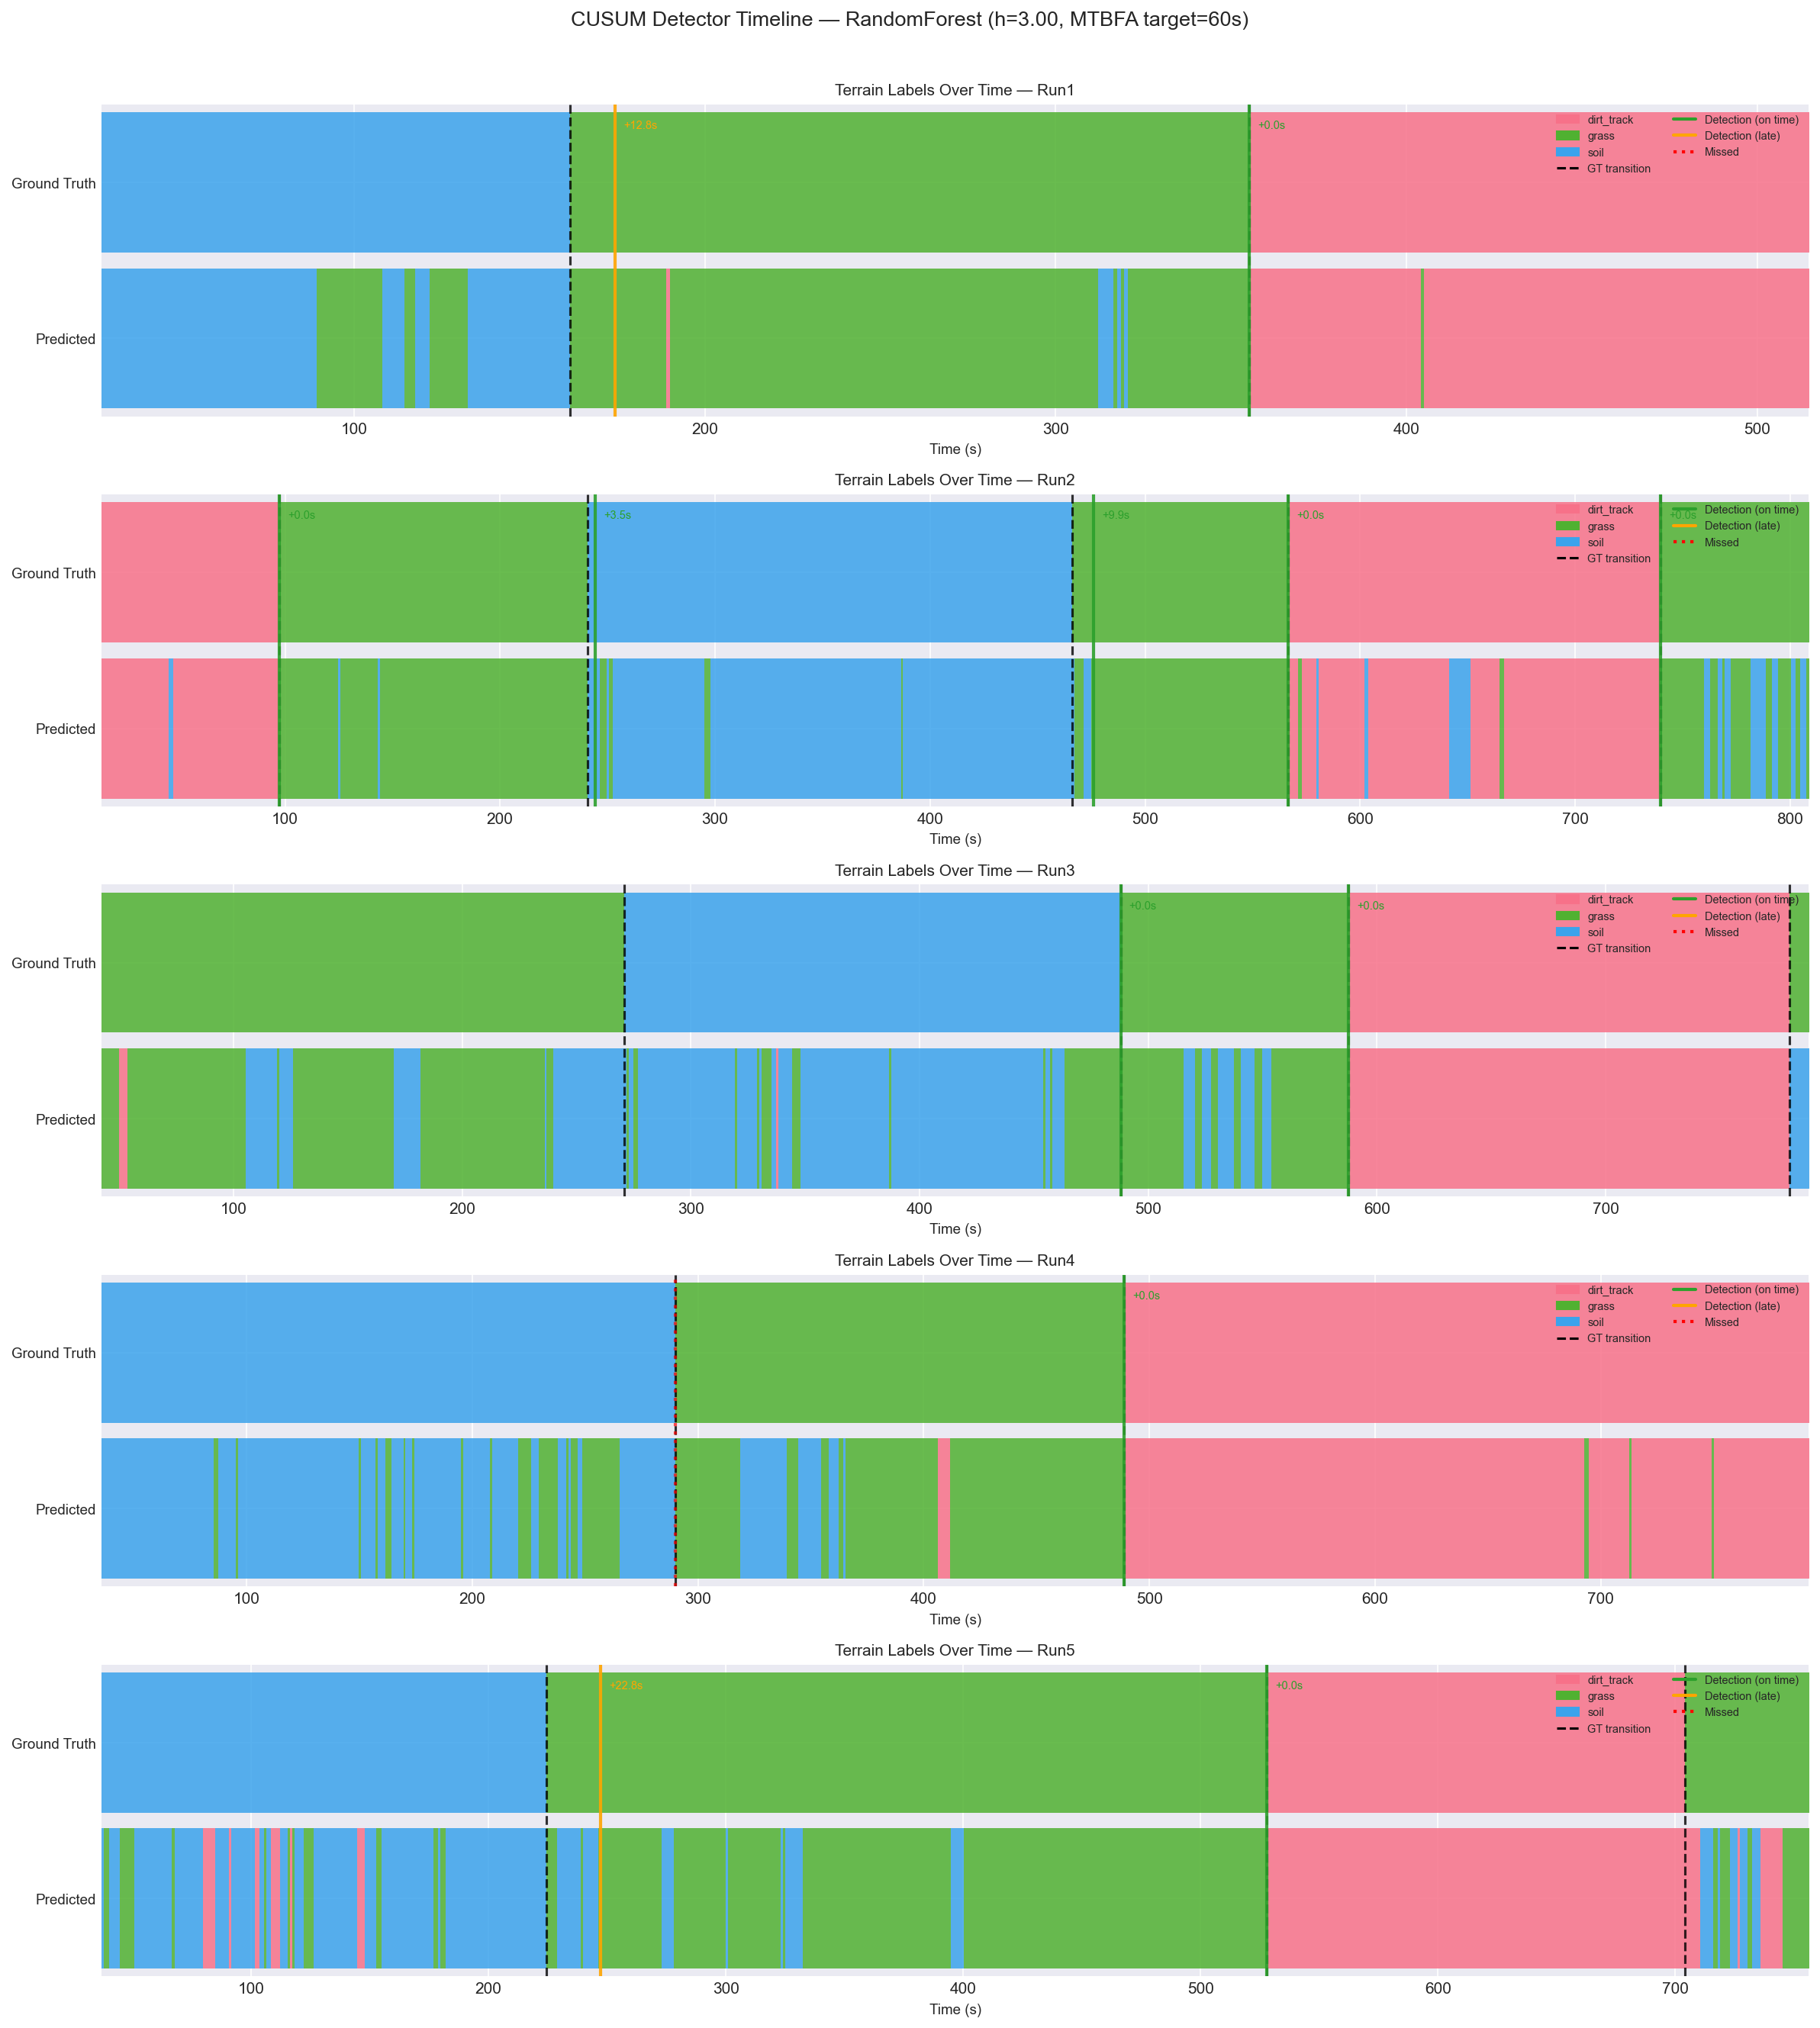
\includegraphics[width=0.85\textwidth]{Pictures/Figures/cusum_timeline_randomforest.png}
    \caption{CUSUM detector trace on the same farm run: the soft posterior (top), the bank of $g_c(k)$ statistics (middle), and the alarm decisions vs.\ the ground-truth transitions (bottom).}
    \label{fig:cusum_timeline}
\end{figure}

\begin{figure}[H]
    \centering
    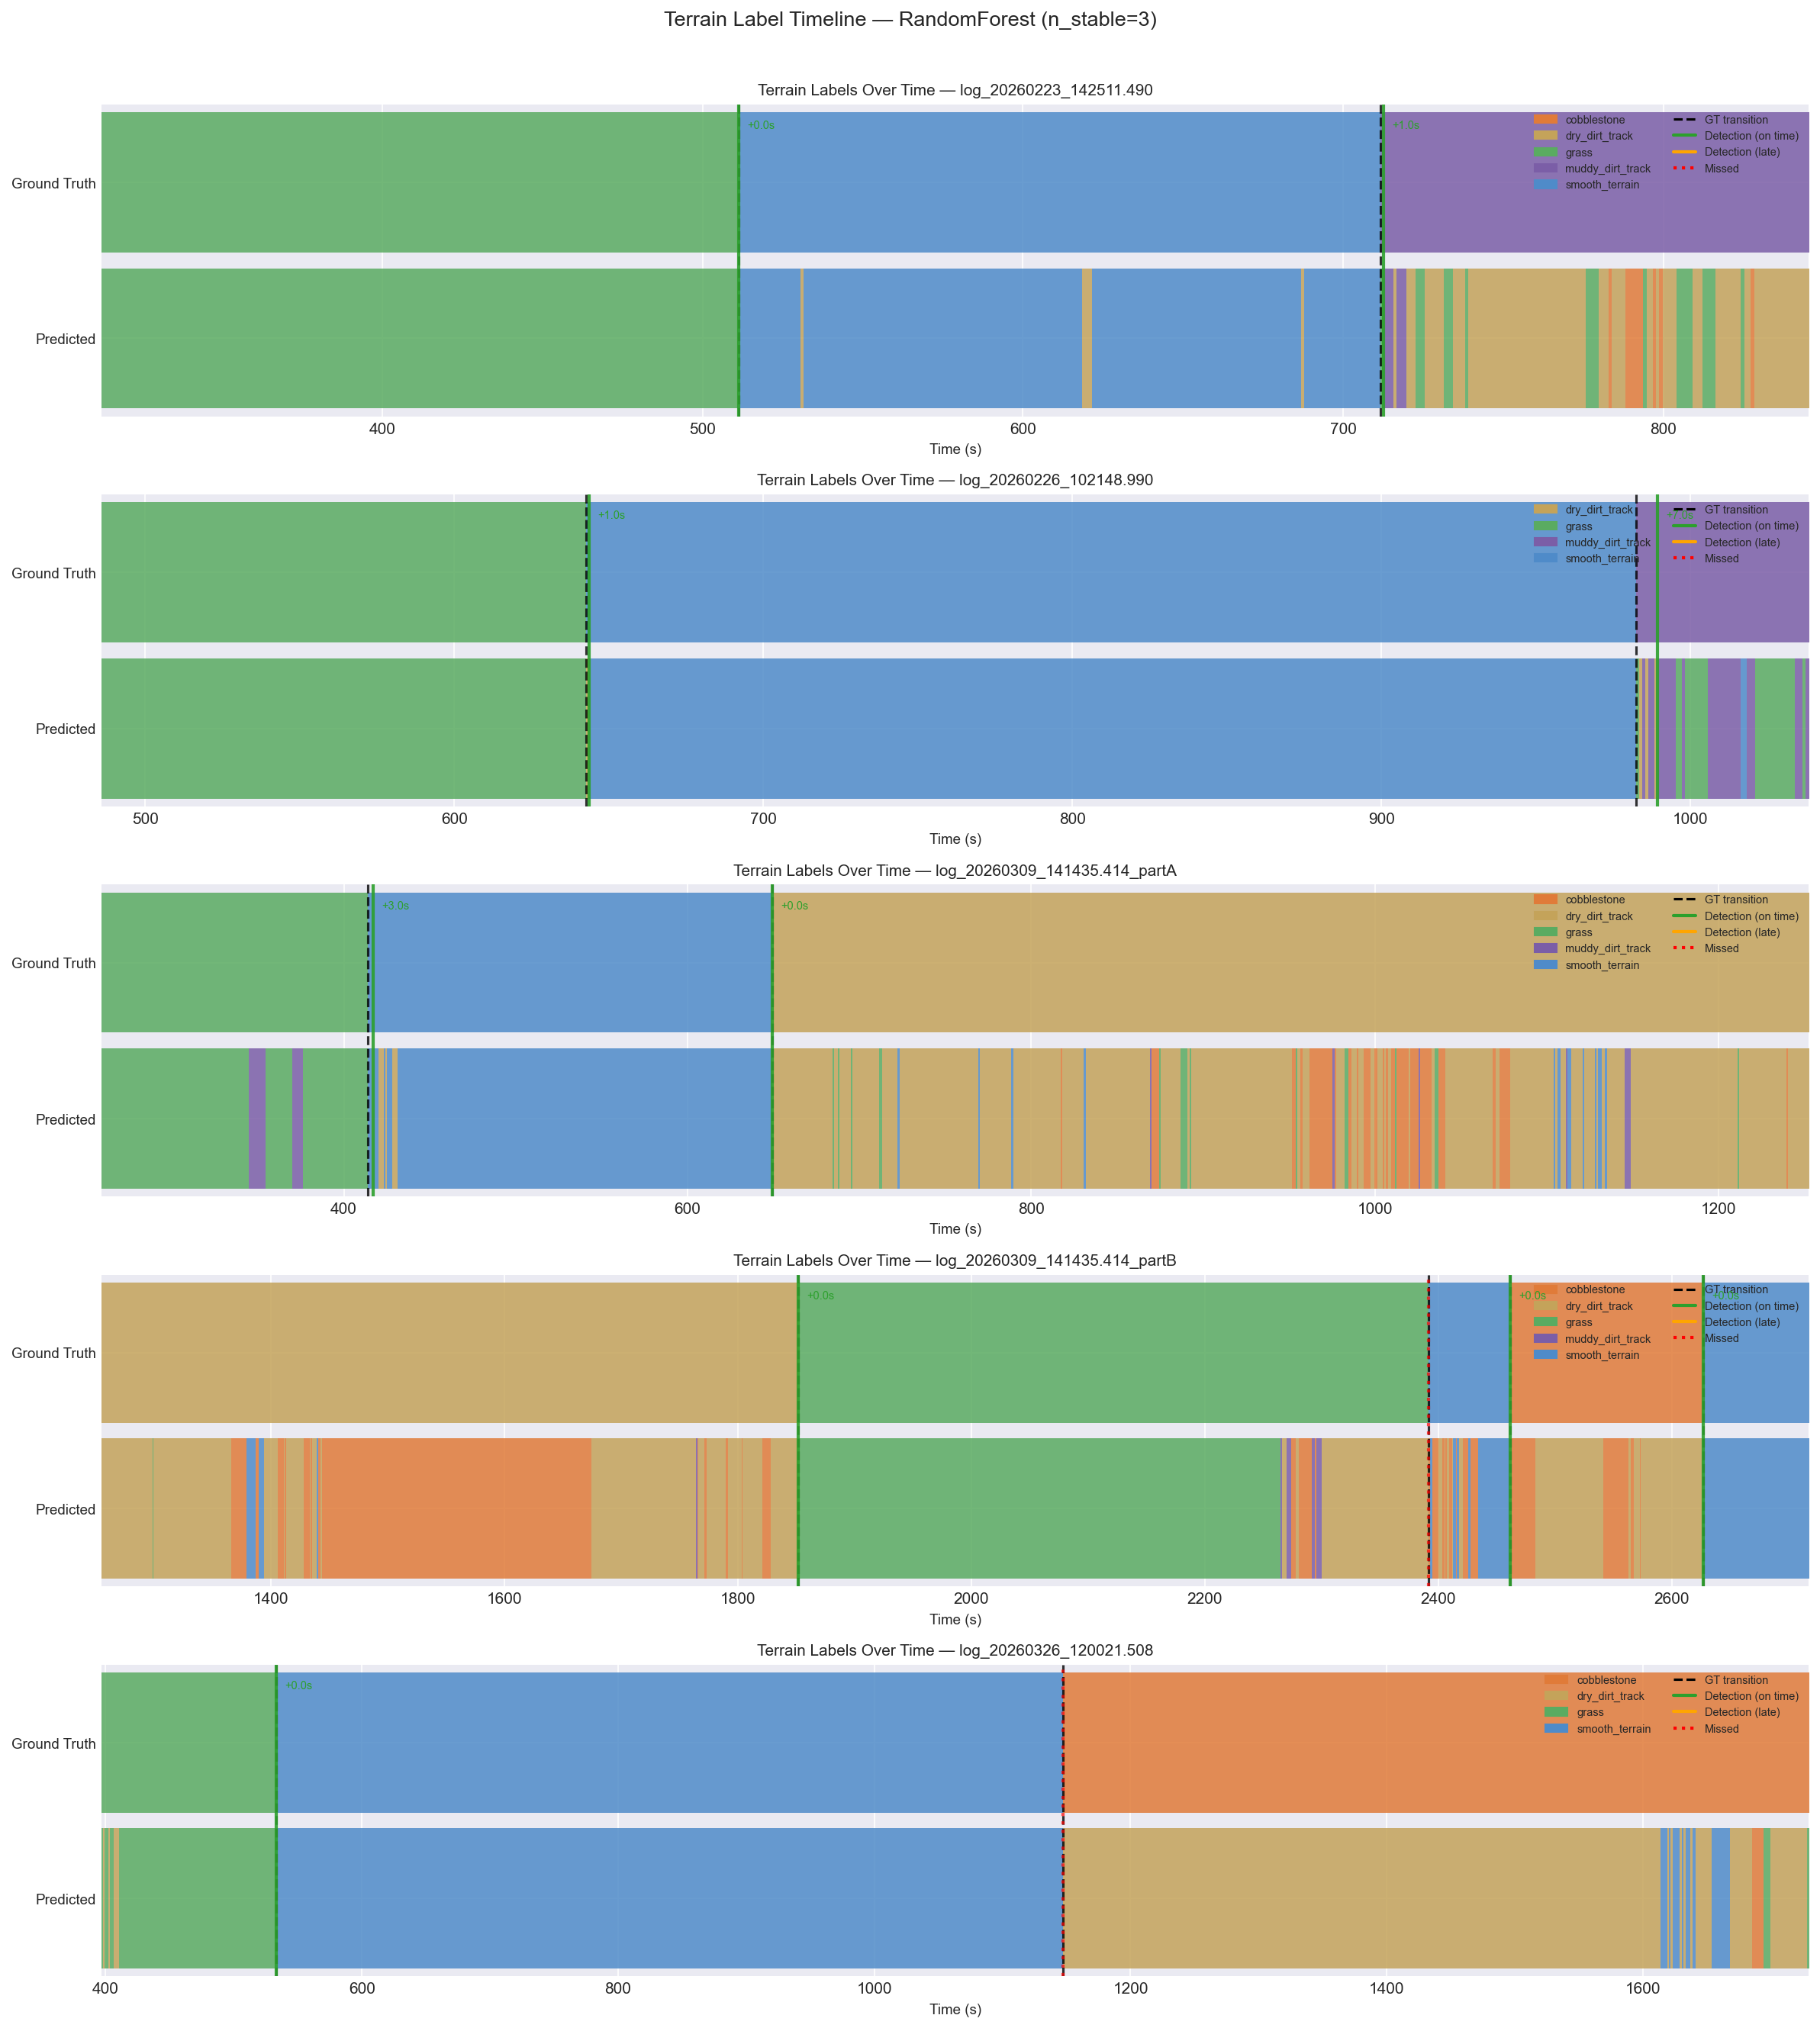
\includegraphics[width=0.85\textwidth]{Pictures/Figures/transition_timelines_randomforest_c.png}
    \caption{Random Forest per-window posterior on a representative campus run, with the $n_{\text{stable}} = 5$ detections overlaid. Shaded bands are ground-truth class segments; vertical lines mark the implicit detector's alarms.}
    \label{fig:transition_timelines_c}
\end{figure}

\vspace{-8mm}
\section{Repository Structure}
\label{app:repo}

The full source code, raw data pipeline notebooks, and results files are available in the project repository. The repository follows the structure described in the project README:

\begin{lstlisting}[language=bash, caption={Repository layout (top level).}]
BSC_Thesis_intrinsic_sensor_analysis/
├── notebooks/       # Sequential Jupyter pipeline (01 through 12)
├── src/             # Reusable Python modules
│   ├── features.py  # Feature engineering
│   ├── io.py        # Sensor log parsing
│   ├── labels.py    # Terrain label assignment
│   ├── preprocess.py# QC, synchronisation, resampling
│   ├── windowing.py # Signal windowing
│   ├── evaluation.py# Model evaluation utilities
│   └── transition.py# Transition detection analysis
├── results/         # Model metrics, tuning outputs (CSV/JSON)
├── reports/         # Per-run QC reports (HTML)
├── data/            # Raw sensor logs (not tracked in git)
└── environment.yml  # Conda environment specification
\end{lstlisting}